\documentclass{standalone}
\usepackage{tikz}

\usetikzlibrary{calc}
\usetikzlibrary{through}


\begin{document}

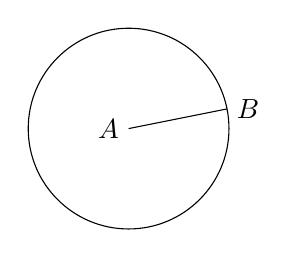
\begin{tikzpicture}
  \coordinate [label=left:$A$]  (A) at ($ (0,0) $);
  \coordinate [label=right:$B$] (B) at ($ (1.25,0.25) $);

  \draw (A) -- (B);

  \node [draw, circle through=(B)] at (A) {};




\end{tikzpicture}

\end{document}
